roughly 2-3 pages
\begin{itemize}
\item explain the model; if any important assumptions are made at this stage, explain why they are reasonable or necessary
\item Explain learning / inference algorithms
\item explaining (perhaps briefly) any necessary preprocessing/postprocessing data acquisition stages (maybe earlier, depending on the project; may also move to the experimental section)
\end{itemize}
Latent Dirichlet Allocation (LDA) treats every document like a collection of words, and presumes that each word in a document is generated by a certain topic. A hidden distribution over topics is assumed to exist for every document. The goal of LDA is to \textit{a)} find a distribution over topics for each document and \textit{b)} find a distribution over words for each topic. Thus, we're looking for two sets of distributions: $\theta_i \sim \text{Dirichlet}(\alpha)$, or a distribution of topics over document $i$, and $\varphi_k \sim \text{Dirichlet}(\beta)$, or a distribution of words over topic $k$. Thus, LDA assumes that some generative model generates a document: for each word position $i,j$ from $i \in$ documents and $j \in$ words$_i$, choose a topic $z_{ij} \sim \theta_i$, then choose a word $w_{ij} \sim \varphi_{z_{ij}}$. \\
In this paper, LDA is extended: instead of finding distributions over topics for every document, topic distributions are learned over genres, where a genre is a non-overlapping set of documents. The difference between regular LDA and genre-LDA can be seen in the graphical models found in figure \ref{fig:graphical-model} (original LDA) and \ref{fig:graphical-model_extended} (genre-LDA). \\
To infer the different distributions, collapsed Gibbs sampling is used (where the distributions $\theta_i$ and $\varphi_k$ are integrated out). The derivation for genre-LDA is similar to, but not exactly the same as the derivation for original LDA. The derivation can be found in section \ref{ref:derivation}.\\
Before any model could be tested, data had to be collected and processed. To do this, a crawler was built that collects song lyrics from \textit{Lyricsmode}\footnote{\texttt{http://www.lyricsmode.com}} by going through the alphabet (with one `letter' for numbers $0-9$), finding the top 100 artists starting with that letter and collecting the first five songs (alphabetically) by that artist. After collecting these lyrics, genre-information was retrieved from \textit{Allmusic}\footnote{\texttt{http://www.allmusic.com}}. The choice of these websites are primarily based on earlier research \cite{felllyrics} that used these websites because of their consistency. \\
After collecting a dataset of $12.102$ lyrics, the data was pre-processed to filter out \textit{a)} punctuation marks and capitalization \textit{b)} non-english lyrics and \textit{c)} low-content, very common words\footnote{For example, 'a', 'by', 'I', 'off', 'were'}, resulting in a dataset of $9.728$ lyrics. These pre-processing steps were done under the assumption that for topic modeling, including common words would create low-information topics that would hardly contribute to the model. Another assumption was made that punctuation and capitalization, while containing useful information regarding language, were not relevant to the kinds of topics that would be found \textbf{HEBBEN WE HIER EEN SOURCE VOOR}. Non-english lyrics were filtered because extraction topics over multiple language would add a lot of noise to the model. Note however, that not \textit{all} non-english words were filtered out (only complete songs in a different language): in many cases, the use of \textit{some} non-english words can say a lot about a genre\footnote{Think of the Latin genre, for example, which turned out to use both english and spanish words quite a lot}. 

\subsection{Derivation}\label{ref:derivation}
\begin{align}
P(w, z, \varphi, \theta | \alpha, \beta, y) &= P(\varphi | \beta)P(\theta | \alpha)P(z | \theta, y)P(w | \varphi, z)\\
\end{align}
Separate probabilities:
\begin{align}
P(\varphi | \beta) &= \prod\limits_{k=1}^K P(\varphi_k|\beta)\\
P(\theta | \alpha) &= \prod\limits_{g=1}^G P(\theta_g|\alpha)\\
P(z | \theta, y) &= \prod\limits_{i=1}^N \prod\limits_{j=1}^{M_i} P(z_{i,j}|\theta_{y_i})\\
P(w | \varphi, z) &= \prod\limits_{i=1}^N \prod\limits_{j=1}^{M_i} P(w_{i,j}|\varphi_{z_{i,j}})\\
\end{align}
Joined together:
\begin{align}
P(w, z, \varphi, \theta | \alpha, \beta, y) &= \prod\limits_{k=1}^K P(\varphi_k|\beta) \prod\limits_{g=1}^G P(\theta_g|\alpha) \prod^N_{i=1}\prod^{M_i}_{j=1} P(z_{i,j}|\theta_{y_i}) P(w_{i,j}|\varphi_{z_{i,j}})
\end{align}
Integrate over joint:
\begin{align}
\int \int P(w, z, \varphi, \theta | \alpha, \beta, y) d\varphi d\theta &= \int \prod\limits_{k=1}^K P(\varphi_k|\beta) \prod^N_{i=1}\prod^{M_i}_{j=1} P(w_{i,j}|\varphi_{z_{i,j}}) d\varphi\\
&\times \int \prod\limits_{g=1}^G P(\theta_g|\alpha) \prod^N_{i=1}\prod^{M_i}_{j=1} P(z_{i,j}|\theta_{y_i}) d\theta
\end{align}
\subsection{Derivation of $\int \prod\limits_{k=1}^K P(\varphi_k|\beta) \prod^N_{i=1}\prod^{M_i}_{j=1} P(w_{i,j}|\varphi_{z_{i,j}}) d\varphi$}
~\\Use $C(k,w)$ as the number of times word $w$ is assigned to topic $k$ in any document.
\begin{align}
\prod\limits_{k=1}^K P(\varphi_k|\beta) \prod^N_{i=1}\prod^{M_i}_{j=1} P(w_{i,j}|\varphi_{z_{i,j}}) d\varphi
\end{align}
\begin{align}
&= \prod\limits_{k=1}^K \int\frac{\Gamma (\sum\limits_{w=1}^V \beta)}{\prod\limits_{w=1}^V \Gamma(\beta)} \prod\limits_{w=1}^V  \varphi_{k}(w)^{\beta-1}  \prod^N_{i=1}\prod^{M_i}_{j=1} \varphi_{z_{i,j}}(w_{i,j})) d\varphi\\
&= \prod\limits_{k=1}^K \int \frac{\Gamma (V \beta)}{(\Gamma(\beta))^V} \prod\limits_{w=1}^V  \varphi_{k}(w)^{\beta-1}  \prod\limits_{w=1}^V \varphi_{k}(w)^{C(k,w)} d\varphi\\
&= \prod\limits_{k=1}^K \int \frac{\Gamma (V \beta)}{(\Gamma(\beta))^V}  \prod\limits_{w=1}^V \varphi_{k}(w)^{\beta + C(k,w) -1} d\varphi\\
&= \prod\limits_{k=1}^K \frac{\Gamma (V \beta)}{(\Gamma(\beta))^V}  \frac{\prod\limits_{w=1}^V \Gamma(C(k,w)-1)}{\Gamma(\sum\limits_{w=1}^V C(k,w)-1))} \int \frac{\Gamma(\sum\limits_{w=1}^V C(k,w)-1))}{\prod\limits_{w=1}^V \Gamma(C(k,w)-1}  \prod\limits_{w=1}^V \varphi_{k}(w)^{\beta + C(k,w) -1} d\varphi\\
&=  \prod\limits_{k=1}^K \frac{\Gamma (V \beta)}{(\Gamma(\beta))^V}  \frac{\prod\limits_{w=1}^V \Gamma(C(k,w)-1)}{\Gamma(\sum\limits_{w=1}^V C(k,w)-1))}\\
&\propto \prod\limits_{k=1}^K \frac{\prod\limits_{w=1}^V \Gamma(C(k,w)-1)}{\Gamma(\sum\limits_{w=1}^V C(k,w)-1))}
\end{align}
\subsection{Derivation of $\prod\limits_{g=1}^G P(\theta_g|\alpha) \prod^N_{i=1}\prod^{M_i}_{j=1} P(z_{i,j}|\theta_{y_i}) d\theta$}
~\\Use $C(g,k)$ as the number of times topic $k$ is assigned to genre $g$ in any document.
\begin{align}
\prod\limits_{g=1}^G P(\theta_g|\alpha) \prod^N_{i=1}\prod^{M_i}_{j=1} P(z_{i,j}|\theta_{y_i}) d\theta
\end{align}
\begin{align}
&= \prod\limits_{g=1}^G \int\frac{\Gamma (\sum\limits_{k=1}^K \alpha)}{\prod\limits_{k=1}^K \Gamma(\alpha)} \prod\limits_{k=1}^K  \theta_{g}(k)^{\alpha-1}  \prod^N_{i=1}\prod^{M_i}_{j=1} \theta_{y_{i}}(k_{i,j})) d\theta\\
&= \prod\limits_{g=1}^G \int \frac{\Gamma (K \alpha)}{(\Gamma(\alpha))^K} \prod\limits_{k=1}^K  \theta_{g}(k)^{\alpha-1}  \prod\limits_{k=1}^K \theta_g(k)^{C(g,k)} d\theta\\
&= \prod\limits_{g=1}^G \int \frac{\Gamma (K \alpha)}{(\Gamma(\alpha))^K}  \prod\limits_{k=1}^K \varphi_{k}(w)^{\alpha + C(g,k) -1} d\theta\\
&= \prod\limits_{g=1}^G  \frac{\Gamma (K \alpha)}{(\Gamma(\alpha))^K}  \frac{\prod\limits_{k=1}^K \Gamma(C(g,k)-1)}{\Gamma(\sum\limits_{k=1}^K C(g,k)-1))} \int \frac{\Gamma(\sum\limits_{k=1}^K C(g,k)-1))}{\prod\limits_{k=1}^K \Gamma(C(g,k)-1}  \prod\limits_{k=1}^K \varphi_{k}(w)^{\alpha + C(g,k) -1} d\theta\\
&=  \prod\limits_{g=1}^G  \frac{\Gamma (K \alpha)}{(\Gamma(\alpha))^K}  \frac{\prod\limits_{k=1}^K \Gamma(C(g,k)-1)}{\Gamma(\sum\limits_{k=1}^K C(g,k)-1))} \\
&\propto  \prod\limits_{g=1}^G   \frac{\prod\limits_{k=1}^K \Gamma(C(g,k)-1)}{\Gamma(\sum\limits_{k=1}^K C(g,k)-1))} 
\end{align}

\subsection{}
~\\ Use $\neg w_{i,j}$ as collection that not uses word from document i at position j. Use $\widetilde{C}$ as a count that does not include word from document i at position j.
\begin{align}
P(z_{i,j} = k | Z_{\neg w_{i,j}}, \alpha, \beta, W, Y) &\propto \frac{\beta + \widetilde{C}(k, w_{i,j})}{V\beta + \widetilde{C}(k)} \times \frac{\alpha + \widetilde{C}(y_i, k)}{K\alpha + \widetilde{C}(y_i)}
\end{align}


\begin{figure}[htp]
	\centering
	\begin{subfigure}[b]{0.5\textwidth}
		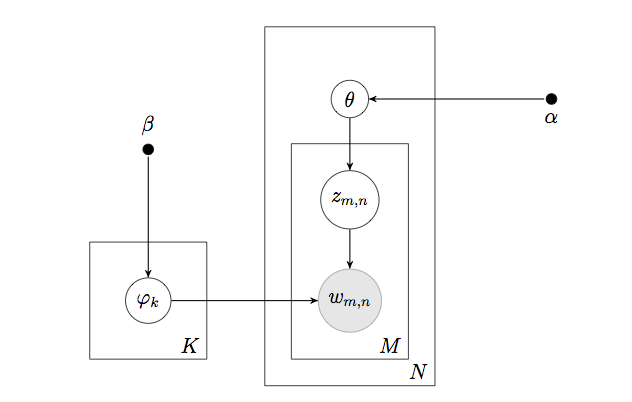
\includegraphics[width=\textwidth]{regular_lda_img}
		\caption{Graphical model for regular LDA}
		\label{fig:graphical-model}
	\end{subfigure}%
        \begin{subfigure}[b]{0.5\textwidth}
		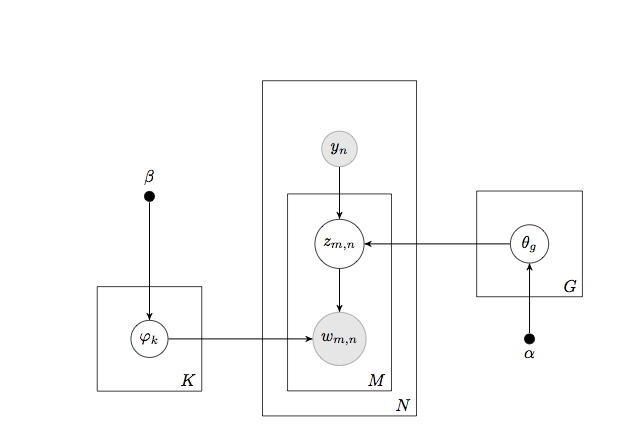
\includegraphics[width=\textwidth]{extended_lda_img}
		\caption{Graphical model for extended LDA}
		\label{fig:graphical-model_extended}
	\end{subfigure}
\end{figure}

